\section{Framework}
The framwork presented in this work allows the user to \textbf{customize} the elements to be used in the design of the \textit{Custom Processor} and \textit{Memory System}, \textbf{explore} custom architectures automatically generated for a given application and \textbf{predict} area, power and latency of such architectures. Figure~\ref{fig:framework} gives an overview of the modules contained in the framework. The framework takes two inputs, the \textit{Configuration Parameters} - described in~\ref{ssec:conf_param} - and an \textit{Application} - detailed in~\ref{ssec:app}. A set of hardware architectures, behaviorally equivalent to the input application, is automatically generated by the framwork. The output is the area, power and latency tradeoff of such architectures. The generated hardware architectures can be used to generate an RTL implementation using the \textit{architectural templates} described in~\ref{sec:arch_template}.
The framework is composed by three modules. The first module - \textit{L2 Model} - models the transfer of the input data between the \textit{Layer 2} memory and the \textit{Layer 1} memory. The \textit{Data Dependency Analysis} performs static analysis on the input application. The last module, \textit{Design Space Exploration}, uses the information extracted by the previous step to procedurally generate hardware architectures.
The rest of this section will describe more in detail the inputs and modules of the framework.
\begin{figure}[tb] 
\centering
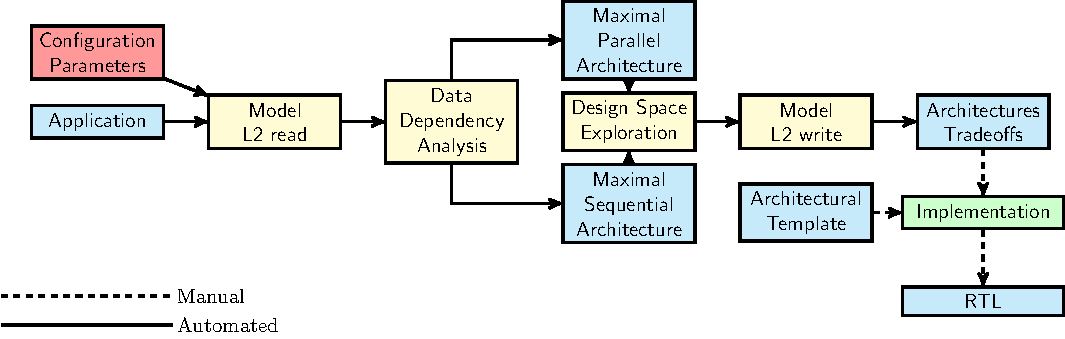
\includegraphics[width=\columnwidth]{images/framework.pdf}
\caption{\small Diagram of the Framework presented in this work.}
\label{fig:framework}
\end{figure}

\subsection{Application}
\label{ssec:app}
The framework performs exact data dependency analysis on the application. This entails that the behaviour of the application needs to be completely specified at compile-time and independent from the input data. Streaming applications meet these requirement and can be analyzed by our framework. Listing~\ref{lst:matrixvec} shows the application source code that will be used for the remainder of this paper. The language that the framework currently supports is C/C++, however the framework uses the LLVM Intermediate Representation CITATION NEEDED, so the support for other languages can be easily added.
\begin{lstlisting}[language=C, caption={Example of input application, C implementation of a matrix vector multiplication.}, label={lst:matrixvec}]
void matrix_vec_kernel(int *A,int *B, int *C){
    int sum;
    for(int i=0;i<DIM2;i++){
        sum=0;
        for(int j=0;j<DIM1;j++){
            sum+=A[i*DIM1+j]*B[j];
        }
        C[i]=sum;
    }
}
\end{lstlisting}

\subsection{Configuration Parameters}
\label{ssec:conf_param}
The second input to the framework is a configuration file. The Configuration file contains a description of the different component to be used in the realization of the hardware architecture, an example is shown in Listing~\ref{conf_file}. Using this file the user can specify the process technology to be used - e.g. 16nm, 28nm - the clock frequency of Layer 1 memory, Layer 2 memory and Custom Processor. The user can moreover specify the datawidth used by the different operators - e.g. multipliers, adders-, and by the Layer 1 and Layer 2 memory. 
Detailed information requred to model the Layer 2 burst accesses are as well contained in this file: the setup latency for write/read accesses, the type of Layer 2 memory to be used -e.g. MRAM, SRAM etc..- and the size of the Layer 2 memory.
\begin{lstlisting}[language=json, caption={Example of input configuration file}, label={lst:conf_file}]
{ 
   "resource_database": { 
	"technology": 16, 
	"clock_frequency": 1000, 
	"bitwidth_adder": 128, 
	"bitwidth_multiplier": 64, 
	"bitwidth_register_file": 128, 
	"type_l2": "tt1v1v85c", 
	"technology_l2": 16, 
	"clock_l2": 800, 
	"bitwidth_l2": 32, 
	"depth_l2":2048, 
	"setup_write_latency_l2":2, 
	"setup_read_latency_l2":2 
   } 
}

\end{lstlisting}

\subsection{Layer 2 Read Model}
The first operation performed by the framework is to compute the transfer time of the input data from the \textit{Layer 2} memory to the \textit{Later 1} memory. A position in Layer 2 memory is given to the input data used by the application, different datastructures are placed in consecutive memory addresses. The entire data transfer is modeled as a single burst read operation to the \textit{Layer 2} memory (see BACKGROUND). The information required to compute the arrival clock time of each input element to the Layer 1 memory is extracted from teh \textit{Configuration Parameters} and performing static analysis on the input \textit{Application}.
Using such information  the exact clock at which each input elements arrives in the Layer 1 memory can be computed with:
$$
AClk_i = rSL + (L2Add_i+1) * (L1B/L2B) * (L1Clk/L2Clk)
$$

Where $rSL$ is the initial latency of a Layer 2 burst read, $L2Add_i$ is the offset of element i from the beginning of the burst access, $L1B$ is the data bitwidth of the Layer 1 memory, $L2B$ is the data bitwidth of the Layer 2 memory, $L1Clk$ is the clock frequency of the Layer 1 memory and $L2Clk$ is the clock speed of the Layer 2 memory.

\subsection{Data Dependency Analysis}
\subsection{Maximal Parallel Architecture and Maximal Sequential Architecture}
\subsection{Design Space Exploration}
\subsection{Layer 2 Write Model}
\subsection{Architecture Tradeoffs}

